\documentclass[12pt, a4paper]{article}
\usepackage[nocompress]{cite}
\usepackage{graphicx}
\usepackage[onehalfspacing]{setspace}
\usepackage{hyperref}
\hypersetup{
    urlcolor=cyan
    }

% extra hierarchielevel
\usepackage{titlesec}
\setcounter{secnumdepth}{4}
\titleformat{\paragraph}
{\normalfont\normalsize\bfseries}{\theparagraph}{1em}{}
\titlespacing*{\paragraph}
{0pt}{3.25ex plus 1ex minus .2ex}{1.5ex plus .2ex}

% YAML highlighting
\usepackage{adjustbox}
\usepackage[dvipsnames]{xcolor}
\usepackage{listings}
\newcommand\YAMLcolonstyle{\color{red}\mdseries}
\newcommand\YAMLkeystyle{\color{black}\bfseries}
\newcommand\YAMLvaluestyle{\color{blue}\mdseries}
\makeatletter
% here is a macro expanding to the name of the language
% (handy if you decide to change it further down the road)
\newcommand\language@yaml{yaml}
\expandafter\expandafter\expandafter\lstdefinelanguage
\expandafter{\language@yaml}
{
  keywords={true,false,null,y,n},
  keywordstyle=\color{darkgray}\bfseries,
  breaklines=true,
  basicstyle=\YAMLkeystyle,                                 % assuming a key comes first
  sensitive=false,
  comment=[l]{\#},
  morecomment=[s]{/*}{*/},
  commentstyle=\color{purple}\ttfamily,
  stringstyle=\YAMLvaluestyle\ttfamily,
  moredelim=[l][\color{orange}]{\&},
  moredelim=[l][\color{magenta}]{*},
  moredelim=**[il][\YAMLcolonstyle{:}\YAMLvaluestyle]{:},   % switch to value style at :
  morestring=[b]',
  morestring=[b]",
  literate =    {---}{{\ProcessThreeDashes}}3
                {>}{{\textcolor{red}\textgreater}}1
                {|}{{\textcolor{red}\textbar}}1
                {\ -\ }{{\mdseries\ -\ }}3,
}
% switch to key style at EOL
\lst@AddToHook{EveryLine}{\ifx\lst@language\language@yaml\YAMLkeystyle\fi}
\makeatother
\newcommand\ProcessThreeDashes{\llap{\color{cyan}\mdseries-{-}-}}
% \lstset{
%   basicstyle=\fontsize{5}\selectfont\ttfamily
% }

\begin{document}

\begin{abstract}
Highly descriptive text-to-face generation to sythesize authentic faces (photofits for criminology purposes) via a GAN. Main project of the  teaching event ``Computer Vision and Deep Learning: Visual Synthesis'' in the summer of 2022 at LMU Munich.
We designed a framework that currently provides two GAN-Models -- cDCGAN and TediGAN -- that are easy to train, evaluate and use to generate photofits. It is implemented in PyTorch and highly configurable to accommodate many test cases. Due to its architecture other models, datasets and metrics can easily be added. We are looking forward to your pull requests.

\end{abstract}
\tableofcontents

\section{Introduction}

\subsection{The Goal of Photofit Creation using GANs}\label{sec:goal}
Our proposed goal for the final project of the "Computer Vision \& Deep Learning: Visual Synthesis" lecture was to train 
existing Generative Adversarial Network (GAN, compare \cite{gan}) models and fine-tune their architectures in respect to generate authentic
and unambiguous samples of real looking faces. These samples should be of such quality that they could be used as
photofits (also phantom images, i.e. pictures representing a person's memory of a criminal's face, compare \cite{photofitDef}).
Even if this common task is already done by phantom sketch artists working for the police or for lawyers, our assumption
is that a GAN creating such photofits could easily outperform every sketch artist in terms of costs, speed, accuracy and photo-realism.
Thus, such a network for the creation of photofits could be a very useful tool for criminology workers.

\subsection{Text-to-Face Synthesis}
Inspired by DALL-E and DALL-E 2 (see \cite{dallE}), our first intention was a text-to-image approach
using two separate models -- analogous to \cite{Xia_2021_CVPR}. On the one hand, we considered to
use a text-encoder model for the embedding of a continuous text describing a criminal's face into the latent space --
such that the semantics of the textual description remain intact. On the other hand, we thought about a GAN or VAE model
creating faces from those latent embeddings.

\subsection{Vector-to-Face Synthesis}\label{sec:vec-to-face}
However, during the execution of the project we changed our plan to only focus on the generation part because of four
crucial arguments. First, the lecture is about visual synthesis and not natural language processing, so our main focus
should be on the creation of images and not on the semantic embedding of continuous text into the latent space.
Second, training a text-encoder and a GAN respectively means twice as much calculation time which is inappropriate for
the relatively short project time. Third, in respect to our described goal (see \ref{sec:goal}) we think that possible
downstream applications would benefit more if the photofit creation is conditioned by vectors with values either 0 or 1
representing the truth value (0=False, 1=True) for each descriptive attribute of an image / a face. Fourth, the attempt
of only generating phantom images based on attribute vectors is sufficient to get a proof of concept and to use such 
model for criminology purposes.

Therefore, to keep things simple and appropriate we decided to focus solely on the principle of using a GAN network --
consisting of two separate models, i.e., a discriminator / encoder and a generator / decoder \cite{gan}.

We finalized a more stable adaption of a classical GAN, namely a Deep Convolutional GAN (DCGAN) which explicitly  uses
convolutional and convolutional-transpose layers in the discriminator and generator respectively \cite{dcgan}.
Since we do not just need to generate random images, but rather images that fit the vectorized description of
a criminals face we conditioned our DCGAN to also use the attribute vector as input -- then it is called a Conditional
DCGAN (CDCGAN).

Moreover, we decided to re-implement another CDCGAN architecture: tediGAN \cite{Xia_2021_CVPR}.
Due to time constraints and some other reasons -- see \ref{sec:tedi} -- we were not able to finalize the
re-implementation of the tediGAN.

\subsection{Related Work}
The number of papers concerning the same topic as ours, text-to-face generation from attributes, is small. We found 17 papers based on a broad range of keywords.
The papers can be divided into two groups. One working with photofits/ forensic or composite sketches and the other with attribute guided face generation.
The first group is mainly focused on generating images from those sketches \cite{6359918, LEI202013, SANNIDHAN2019452}. This is not what we intended to do. 
The other group employs networks to generate faces from attributes which matches our goal \cite{Xia_2021_CVPR,Lu_2018_ECCV,9117185,9320290,9412022,8462648,Gecer_2018_ECCV,8606936,9146375,Bodla_2018_ECCV,NIPS2016_b1301141,gauthier2014conditional,Xiao_2018_ECCV}.
We selected three papers which give relevant information for our project. First ``TediGAN: Text-Guided Diverse Face Image Generation and Manipulation'' by Xia 
et al. published in 2021\cite{Xia_2021_CVPR}. The second paper is ``Attribute-Guided Sketch Generation'' by Tang et al. published in 2019\cite{Tang}, which is 
the only paper bringing both aspects together. And the DCGAN paper from Goodfellow et al.\cite{dcgan}.

\section{Main}
\subsection{Dataset}
\subsubsection{Suitable Datasets}\label{SuitableDatasets}
During our research in the project planning phase we stumbled across various datasets that could be useful to us in
terms of their properties. Some examples of datasets containing faces and corresponding descriptions or attributes are:
\begin{itemize}
    \item \href{https://mmlab.ie.cuhk.edu.hk/projects/CelebA.html}{celebA}, see \cite{celebA}
    \item \href{http://mmlab.ie.cuhk.edu.hk/projects/CelebA/CelebAMask_HQ.html#:~:text=CelebAMask\%2DHQ\%20is\%20a\%20large,facial\%20attributes\%20corresponding\%20to\%20CelebA}{celebA HQ}, see \cite{CelebAMask-HQ}
    \item \href{http://vis-www.cs.umass.edu/lfw/}{LFW}, see \cite{LFW}
    \item \href{https://github.com/pterhoer/MAAD-Face}{MAAD-Face}, see \cite{DBLP2}
\end{itemize}

Nevertheless, these datasets are not made for criminology purposes, and so they do not perfectly fit our approach of
generating photofits. This has two main reasons.

First, baseline face datasets are mainly constructed for face recognition applications. On the one hand, as the authors
of MAAD-Face outline, this leads to the consequence that datasets like
celebA or LFW indeed contain a large amount of face images, but struggle with the overall annotation correctness and the total number of attributes.
On the other hand, MAAD-Face aims to be better in those terms by merging
face image datasets with their attribute annotations together and check their correctness by a human evaluation.

Second, as we already expected beforehand and was confirmed during the project execution, such relatively low numbers of
distinctive attributes (compare table, TODO) would not fit the demand for accuracy needed for phantom image creation.
Moreover, considering the 40 attributes of celebA one can see that
there is some redundancy and incompleteness within -- e.g. one extra attribute for each Black\_Hair, Blond\_Hair,
Brown\_Hair, and Gray\_Hair, but there is no attribute like  Red\_Hair.

TODO table with dataset stats

\subsubsection{Our Decision}
Comparing the statistics of the datasets from above, we concluded to initially use a set that has a good trade-off
between the total number of face images and the total number of distinctive attributes. Even if they are not perfectly
fitted for criminology purposes, our assumption is that if the concept of attribute-conditioned face generation works on
one of these datasets, it will also work on more accurate datasets that could be developed especially for the task of
photofit creation in the future. And especially, it will work better on a better suited dataset.

Even if MAAD-Face aims to be better than
celebA and LFW, we decided to
use celebA. MAAD-Face has too many images as if we could manage to train our GAN on it in the give time frame of the project and LFW has too few images.

\subsection{Framework}
\subsubsection{Architecture / Structure}
In respect of a uniform and consistent setting for the experiments on different models and datasets we decided to
implement a highly configurable and extendable framework.
Having such a framework that is easily and uniformly executable for different combinations of configurations is a very
powerful tool -- especially regarding adapted experiments / work in the future.

The key features consist of a clear experiment configuration via a yaml-file (1), the simple extensibility of the models,
datasets and metrics (2) as well as a complete and useful documentation of the results (3).

Regarding the key feature (1), a detailed documentation on such a configuration file can be found below --
see \ref{sec:config}.
On the program start the specified configuration file is parsed in the module misc/main.py.
For the cases of any misconfiguration an error designed especially for such cases -- compare misc/error.py -- will be
thrown and the program stops.

The key feature (2) led to the decision to implement a predominantly generic module training.py which holds a
parent-child class-structure that can handle any learning or evaluation of a photofit creation model based on machine
learning.
The inheritance concept represents the three fundamental execution types / modes of the framework, namely train
(short for training, corresponding class: Trainer), eval (short for evaluation, corresponding class: Evaluator) and gen
(short for generation, corresponding class: Creator).
Moreover, the training of a pretrained model can be continued providing a path to the pretrained model and epoch
checkpoint.
The huge benefit of this key feature is the re-usability of pretrained models as well as their generic evaluation and
the generation of photofits.

The evaluation of training results is easy due to key feature (3).
The module main.py creates a clearly arranged directory with an unique name -- i.e., the timestamp of the execution --
holding all results (e.g., samples), statistics (e.g., losses and probabilities), model-checkpoints, the logs and a
snapshot of the configuration file from the beginning of the execution.

\subsubsection{CDCGAN}
As already mentioned in \ref{sec:vec-to-face}, a CDCGAN is a GAN using convolutional and convolutional-transpose layers
-- compare \cite{dcgan}.
We implemented a classical approach in the module model/cdcgan.py using a discriminator model and a generator model --
compare \cite{gan}.
The discriminators job is to distinguish between real and fake samples whereas the generators job is to produce samples
that make the discriminator believe they are real.
Since our goal is the vector-to-face synthesis we also conditioned both of the models so they are able to learn the
context of an image and its attributes.
So the generator will especially be able to sample images from the latent space that fit a given attribute vector.
To make the network architecture work on the celebA dataset we had to rethink the whole layer architectures and the
principle of concatenating the attribute vector with the images and the noise vector in the discriminator and generator
respectively.
The final architecture of our CDCGAN is represented in \ref{} TODO.

\subsubsection{TediGAN}
\label{sec:tedi}
TediGAN is a GAN and Framework proposed by Xia et al. To generate their images they use an inverted pretrained StyleGAN. The Framework includes multiple options to choose between layers and StyleGANs. 
Unfortunately neither the git-repository nor their paper provides clear information which was their final and best version. The framework also uses config files in an incomprehensible way. We tried to 
implement the network into our framework but couldn't get it to start training. Problems we encountered were the configs, which we replaced by one single choice. They also wrote certain layers in C++ and 
Cuda which we initially struggled with but in the end got to work. But then we encountered a dimension error which was weird due to all shapes matching one another. To resolve the dimension error we 
logged and followed the flow of the images in the fit() method. To get further information about the configs we contacted the authors but never got an answer.
To check for implementation errors we also cloned their repository and tried executing their proposed way to train with their framework. It failed to start due to missing config options.

\subsubsection{Metrics}\label{metrics}
Regarding the metrics we orientated us among the most frequently used ones from the papers we read and chose the four most relevant. 
In regard of image generation normal metrics, like accuracy, are very relative and should not be used due to their lack of information value. In most ML context this would not apply. When training a discriminator to decide if a picture is from a real dataset or generated from the GAN's generator, the scores most of the time do not result in ``good'' as in real images. A human could easily differentiate both. 
So for image generation and their realness one should use one of the following metrics for evaluating the new images: on the overall similarity the Fréchet Inception Distance (FID), patch similarity (Learned Perceptual Image Patch Similarity, LPIPS), Blind/Referenceless Image Spatial Quality Evaluator (BRISQUE) or a metric using a discriminator specifically trained for this task, where you know the results are satisfactory.
FID calculates the Fréchet distance which is originally used for the distance between curves of functions but can also be used for the probability distribution, in our case two datasets \cite{NIPS2017_8a1d6947}. $$d^2 = |\mu_X - \mu_Y|^2 + tr(\sum_X + \sum_Y - 2 (\sum_X \sum_Y)^{\frac{1}{2}})$$
One way to check patch similarity between two images is using LPIPS. This metric is based on comparing similarity of activations in a predefined network. A lower score is better \cite{DBLP}. 
To check overall spatial image quality one could use BRISQUE. It checks for e.g. noise or blurriness. 
Kynkäänniemi et al. propose an improved precision and recall framework, which can additionally to precision and recall scores also calculate a realism score. They use a StyleGAN to evaluate a set of images \cite{NEURIPS2019_0234c510}.
Some papers also use humans to give feedback on realness of generated images, which can be unreliable and the number of samples to review is limited \cite{Xia_2021_CVPR}.

In our framework we implemented FID, LPIPS and BRISQUE. Kynkäänniemi's metric is implemented in an outdated version of TensorFlow. 
While implementing each metric a few key differences appeared which do not get clarified by any paper: e.g. LPIPS calculate the similarity between two pictures. 
But are they chosen at random or is an order selected in the beginning and then those images get compared? We chose to generate images based on the same attribute-vectors and compare those to one another.

\subsubsection{Experiments}

\paragraph{Configuration}
\label{sec:config}

Below you can see a template configuration file for the training of the CDCGAN model on the celebA dataset.
This example configuration outlines that our framework is highly configurable. 

\begin{lstlisting}[language=yaml,
    basicstyle=\tiny,
]
mode: train # (train / eval / gen)
log_level: 20 # CRITICAL = 50, ERROR = 40, WARNING = 30, INFO = 20, DEBUG = 10, NOTSET = 0
device: cpu # (cuda / cpu / auto)
experiment_path: ..\experiments # directory where the results should be persisted
epochs: 500 # number of epochs
num_imgs: 20 # how many randomly generated images should be saved
predefined_images: {
    max: [0,0,1,1,0,0,0,0,0,1,0,0,0,0,0,1,0,0,0,1,1,1,0,0,1,0,1,0,0,0,0,1,0,0,0,0,0,0,0,1],
    daniel: [0,1,1,1,0,0,0,1,0,0,0,1,0,0,0,0,0,0,0,0,1,1,0,0,1,0,1,0,1,0,0,1,0,0,0,0,0,0,0,1]} # predefined attribute vectors for the image generation

frequencies:
  save_freq: 1 # (i.e. how often should the model checkpoint be saved, in epochs)
  gen_freq: 1 # (i.e. how often should test images be generated, in epochs)

dataloader:
  dataset: celebA # name of the dataset
  size_fraction: 4 # 4 means use 1/4th of the dataset
  batch_size: 128 # number of images processed in one forward-call of the models
  image_size: 64 # image size (64 x 64)

model:
  name: CDCGAN # name of the mode
  pretrained_path: ../experiments/train/template-CDCGAN-train/2022-08-10-10-08-52 # empty if start from scratch
  start_epoch: 0 # empty if start from scratch
  criterion: BCELoss # name of the loss function
  optimizer: Adam # name of the optimizer
  learning_rate: 0.001 # learning rate for the optimizer
  parameters:
    dropout: 0.2 # how many neurons should be deactivated during forwarding
    alpha: 0.1 # model specific parameter
    beta1: 0.1 # model specific parameter
    ngf: 64 # number of features in the generator
    ndf: 64 # number of features in the discriminator
    z_channels: 128 # size of the noise vector
    use_spectral_norm: False # whether to wrap convolutional layers in spectral_norm or not
\end{lstlisting}


\paragraph{Results}
We planned the training process to run every model variation at least once for 100 epochs on a quarter of the celebA dataset. Each Training run took between 9 and 11 hours. After this preliminary phase we looked at the generated images, loss, accuracy and metrics of our networks. We then decided that a dropout of 0.3 or 0.5 and spectral convolution layer were beneficial. Thus we ran those on the entire dataset size. Those runs took 12 hours on our system. We also tried out running a model for 200 epochs but noticed mode collapse happened every time. Mode collapse also happend when restarting on an epoch without collapse.

Percieved realness is an intuitive score between 0 and 5: $0\widehat{=} $ just noise, $1\widehat{=} $ shape recognizeable, $\ge 2\widehat{=} $ can recognize faces, $\ge 3\widehat{=} $ face with noise, $\ge 4\widehat{=} $ face with small artifacts, $5 \widehat{=} $ real faces without errors. DS\_size means dataset size.
\begin{table}
\centering
\resizebox{\textwidth}{!}{%
\begin{tabular}{|l|l|l|l|l|l|l|}
    \hline
    network                                                                             & \begin{tabular}[c]{@{}l@{}}accuracy real\\ accuracy fake before disc\\ accuracy fake after disc\end{tabular} & \begin{tabular}[c]{@{}l@{}}loss real\\ loss fake\\ loss gan\end{tabular} & FID     & LPIPS & BRISQUE & \begin{tabular}[c]{@{}l@{}}percieved realness\\ (between 0 and 5)\end{tabular} \\ \hline
    \begin{tabular}[c]{@{}l@{}}dropout=0\\ spectral=False,\\ DS\_size=1/4\end{tabular}  & \begin{tabular}[c]{@{}l@{}}0.994\\ 0.006\\ 0.0007\end{tabular}                                               & \begin{tabular}[c]{@{}l@{}}0.0072\\ 0.0074\\ 13.868\end{tabular}         & 339.957 & 0.379 & 16.946  & 1                                                                              \\ \hline
    \begin{tabular}[c]{@{}l@{}}dropout=0\\ spectral=True\\ DS\_size=1/4\end{tabular}    & \begin{tabular}[c]{@{}l@{}}0.968\\ 0.031\\ 0.009\end{tabular}                                                & \begin{tabular}[c]{@{}l@{}}0.046\\ 0.411\\ 6.815\end{tabular}            & 139.774 & 0.161 & 34.917  & 2.5                                                                            \\ \hline
    \begin{tabular}[c]{@{}l@{}}dropout=0.2\\ spectral=False\\ DS\_size=1/4\end{tabular} & \begin{tabular}[c]{@{}l@{}}0.894\\ 0.105\\ 0.062\end{tabular}                                                & \begin{tabular}[c]{@{}l@{}}0.210\\ 0.211\\ 6.640\end{tabular}            & 124.138 & 0.156 & 31.376  & 2.5                                                                            \\ \hline
    \begin{tabular}[c]{@{}l@{}}dropout=0.2\\ spectral=True\\ DS\_size=1/4\end{tabular}  & \begin{tabular}[c]{@{}l@{}}0.969\\ 0.028\\ 0.062\end{tabular}                                                & \begin{tabular}[c]{@{}l@{}}0.0418\\ 0.0356\\ 6.6371\end{tabular}         & 168.228 & 0.265 & 44.231  & 2                                                                              \\ \hline
    \begin{tabular}[c]{@{}l@{}}dropout=0.3\\ spectral=False\\ DS\_size=1/4\end{tabular} & \begin{tabular}[c]{@{}l@{}}0.826\\ 0.180\\ 0.129\end{tabular}                                                & \begin{tabular}[c]{@{}l@{}}0.393\\ 1.003\\ 3.766\end{tabular}            & 139.830 & 0.294 & 29.432  & 1                                                                              \\ \hline
    \begin{tabular}[c]{@{}l@{}}dropout=0.3\\ spectral=True\\ DS\_size=1/4\end{tabular}  & \begin{tabular}[c]{@{}l@{}}0.952\\ 0.046\\ 0.022\end{tabular}                                                & \begin{tabular}[c]{@{}l@{}}0.0612\\ 0.0616\\ 5.7318\end{tabular}         & 173.991 & 0.205 & 41.228  & 1                                                                              \\ \hline
    \begin{tabular}[c]{@{}l@{}}dropout=0.3\\ spectral=True\\ DS\_size=1\end{tabular}    & \begin{tabular}[c]{@{}l@{}}0.999\\ 7.308\\ 7.210\end{tabular}                                                & \begin{tabular}[c]{@{}l@{}}1.12\\ 0.0\\ 44.171\end{tabular}              & 218.512 & 0.271 & 28.791  & 1                                                                              \\ \hline
    \begin{tabular}[c]{@{}l@{}}dropout=0.5\\ spectral=False\\ DS\_size=1/4\end{tabular} & \begin{tabular}[c]{@{}l@{}}0.506\\ 0.501\\ 0.496\end{tabular}                                                & \begin{tabular}[c]{@{}l@{}}0.750\\ 1.737\\ 0.768\end{tabular}            & 145.371 & 0.327 & 73.911  & 1                                                                              \\ \hline
    \begin{tabular}[c]{@{}l@{}}dropout=0.5\\ spectral=True\\ DS\_size=1/4\end{tabular}  & \begin{tabular}[c]{@{}l@{}}0.821\\ 0.179\\ 0.131\end{tabular}                                                & \begin{tabular}[c]{@{}l@{}}0.263\\ 0.262\\ 3.003\end{tabular}            & 141.477 & 0.353 & 45.244  & 2                                                                              \\ \hline
    \begin{tabular}[c]{@{}l@{}}dropout=0.5\\ spectral=True\\ DS\_size=1\end{tabular}    & \begin{tabular}[c]{@{}l@{}}0.929\\ 0.070\\ 0.048\end{tabular}                                                & \begin{tabular}[c]{@{}l@{}}0.108\\ 0.107\\ 5.587\end{tabular}            & 135.339 & 0.213 & 64.889  & 1.5                                                                            \\ \hline
\end{tabular}
}
\end{table}

When deciding which network was the best you can proceed based on statistics, on the proposed metrics or visually judgeing the generated images per epoch and foremost the last epoch. 
One could also proceed based on theoretically taught metrics, e.g. generator accuracy and discriminator accuracy should meet at 0.5 or at least converge against each other. In this case the network with spectral convolution and dropout value being 0.3 is supposed to be the best one. But even on first glance every human would be able to differentiate between real and fake images. 
Running metrics proposed in the metrics section:\ref{metrics}, on trained networks resulted in some mismatching images even compared to the generated ones in the last epoch. When going on the metrics FID is probably the most meaningful. The best network according to this metric would be with dropout 20\% and without a spectral convolutional layer. Some generated images are just noise. Every now and then you can recognize parts of a face but the rest is still just random artifacts. So the results are only partly acceptable. The network with 0\% dropout without a spectral layer is correctly the worst variant with the highest FID score of 339.957 and images looking like weird color sprinkles, see figure \ref{fig:worstImage}.
When looking through all images of every last epoch the best network is tied between (dropout=50\%, spectral=True, DS\_size=1/4) and (dropout=0\%, spectral=True, DS\_size=1/4). But even these images still have some artifacts in the image or on the face, the images are highly noisy around the face. 
Sometimes the network tries to generate two faces into one, fig.\ref{fig:twoFacesInOne}. 
Also our networks seemed unable to learn the difference between certain attributes. 
E.g. they are not able to generate blonde people fig.\ref{fig:blonde} or they put sunglasses on people fig.\ref{fig:sunglasses}. The sunglasses phenomenon happend with a constant c-vector which didn't specify it and the glasses would appear and disappear epoch-wise.
A relative good result is fig.\ref{fig:relgood1} and fig.\ref{fig:relgood2}. But even those fake images are distinguishable compared to the used dataset.
\begin{figure}
    \makebox[\textwidth][c]{
\includegraphics[width=0.25\textwidth]{./results/predef_img_max_7_3specfull_85.png}}%
    \caption{Mutliple eyes in one face.}
    \label{fig:twoFacesInOne}
\end{figure}
\begin{figure}
    \makebox[\textwidth][c]{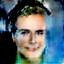
\includegraphics[width=0.25\textwidth]{./results/predef_img_max_2_spectral2quarter99.png}}
    \caption{Network struggles to make entire head of hair in blonde.}
    \label{fig:blonde}
\end{figure}
\begin{figure}
    \makebox[\textwidth][c]{
\includegraphics[width=0.25\textwidth]{./results/predef_img_max_2_spectral4full.png}}
    \caption{Network puts glasses on face.}
    \label{fig:sunglasses}
\end{figure}
\begin{figure}
    \makebox[\textwidth][c]{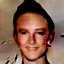
\includegraphics[width=0.25\textwidth]{./results/good-4-spectral-full.png}}
    \caption{Relatively good picture after 100 epochs. Dropout=0.5, spectral=True}
    \label{fig:relgood1}
\end{figure}
\begin{figure}
    \makebox[\textwidth][c]{
\includegraphics[width=0.25\textwidth]{./results/predef_img_daniel_1_spectral4quarter.png}}
    \caption{Relatively good picture after 100 epochs. Dropout=0.5, spectral=True}
    \label{fig:relgood2}
\end{figure}
\begin{figure}
        \makebox[\textwidth][c]{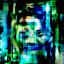
\includegraphics[width=0.25\textwidth]{./results/29.jpg}}
        \caption{Really bad result.}
        \label{fig:worstImage}
\end{figure}

\section{Conclusion}
In this chapter we want to conclude an reflect on the results and things we noticed while implementing or experimenting.
\subsection{Datasets}
First, we observed some defects in the training images that some faces were stretched or had some artifacts e.g see images\ref{fig:badDatasetImage}, \ref{fig:badDatasetImage2} and \ref{fig:badDatasetImage3}.
Second, the attributes are redundant and incomplete. E.g. 4 attributes for hair color, Red\_Hair is completely missing. 
Third it would be better if the direction in which a person looks, would only be straight ahead or be labeled. fig.\ref{fig:wrongDirectionImage} and fig.\ref{fig:wrongDirectionImage2}.
Four, due to the small time frame we were unable to run our experiments with the other datasets mentioned above, chapter: \ref{SuitableDatasets}.
Fifth, often it is the case that many faces match to one and the same attribute-vector so for criminology purposes one should consider to use a dataset with a much larger attribute-vector.
\begin{figure}
    \makebox[\textwidth][c]{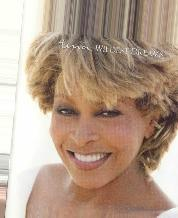
\includegraphics[width=0.25\textwidth]{./results/000111.jpg}}
    \caption{Example image from dataset with artifacts.}
    \label{fig:badDatasetImage}
\end{figure}
\begin{figure}
    \makebox[\textwidth][c]{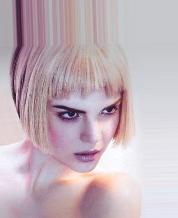
\includegraphics[width=0.25\textwidth]{./results/000347.jpg}}
    \caption{Example image from dataset with artifacts.}
    \label{fig:badDatasetImage2}
\end{figure}
\begin{figure}
    \makebox[\textwidth][c]{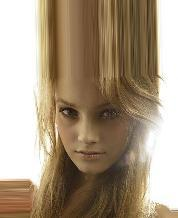
\includegraphics[width=0.25\textwidth]{./results/000812.jpg}}
    \caption{Example image from dataset with artifacts.}
    \label{fig:badDatasetImage3}
\end{figure}
\begin{figure}
    \makebox[\textwidth][c]{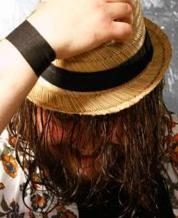
\includegraphics[width=0.25\textwidth]{./results/000199.jpg}}
    \caption{Example image from dataset: person looking down and face hidden behind hair and hat.}
    \label{fig:wrongDirectionImage}
\end{figure}
\begin{figure}
    \makebox[\textwidth][c]{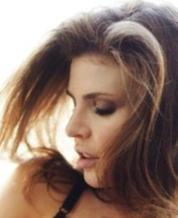
\includegraphics[width=0.25\textwidth]{./results/000240.jpg}}
    \caption{Example image from dataset: person from the side.}
    \label{fig:wrongDirectionImage2}
\end{figure}

\subsection{Mode Collapse}
Mode Collapse is a common problem when working with GANs \href{https://machinelearning.wtf/terms/mode-collapse/}{(see this article)}. 
Normally a GAN is considered successful if its samples can fool a discriminator and the generator samples diverse images with a distribution like in the real world. 
This means that given an attribute-vector $c$ the GAN should sample different images. Mode collapse happens if the GAN starts to produce the same image again and again for the same $c$
because it successfully fools the discriminator. An example can be seen in fig.\ref{fig:modecollapse}.
The image is a result after 100 epochs with spectral convolutions and 0\% dropout. As you can see the images all look alike and there is no real difference between them. Also we have checked some attribute-vectors 
and as one might assume there are multiple individuals annotated with the same vector. This seems pretty plausible with a dataset of more than 200 thousand images and a relatively small attribute-vector size of 40. Therefore 
we also expected our GAN to sample different images for the same $c$. However thinking of photofits it could be useful to run into mode collapse, here a specific vector should always lead to the same result.
\begin{figure}
    \makebox[\textwidth][c]{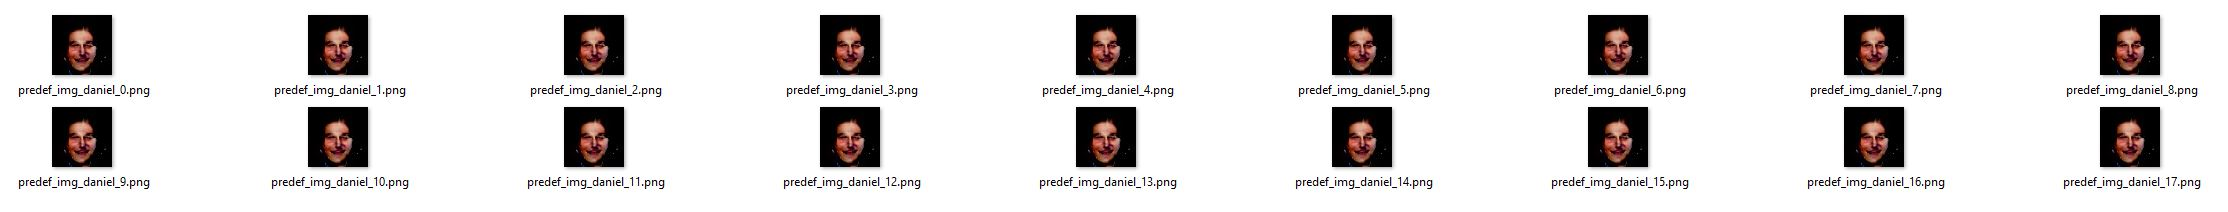
\includegraphics[width=\textwidth]{./results/modecollapse.JPG}}
    \caption{Example for mode collapse after 100 epochs.}
    \label{fig:modecollapse}
\end{figure}
\subsection{Image size}
For time and hardware reasons we opted to scale the dataset images to size 64 by 64. We assume that we can achieve better results with bigger sized images due to a higher detail level.

\subsection{More time + GPU-power}
With more time and better hardware (maybe even multiple GPUs) we would have done more extensive testing and more training runs, and prove our hypothesis that a more detailed dataset and larger images lead to a general improvement.

\section{Future Work}
As described in the conclusion we would like to train our GAN on other datasets, section \ref{SuitableDatasets}, and with a larger image size than 64 by 64. 
Also the development of a new dataset specialized for criminology purposes would be helpful for us and downstream applications.
Such a dataset should contain much more than fourty attributes, we assume about 200 would be a good starting point. Moreover the images of the dataset should not include bad samples as pointed out above but only passport photo should be included.
Regarding mode collapse it would be interesting if someone could use this phenomenon for photofit generation.
\section{Collaboration}
We started our project commonly by exchanging our ideas, thoughts and how to approach our topic.
We did most of the implementation of our framework by pair programming. Certain parts which only one of us did are marked in the table below.
\begin{table}[h]
\centering
    \begin{tabular}{|c|c|}
        \hline
        Implementation & Person \\        
        \hline
        main.py error.py log.py & Max\\
        CDCGAN.py & 70-30 Max-Daniel\\
        TediGAN.py & 30-70 Max-Daniel\\
        Metrics.py & Daniel\\
        Config.py & Max\\
        Dataset.py & Max\\
        Training.py & 80-20 Max-Daniel\\
        Experiments & Daniel\\
        \hline
    \end{tabular} 
\end{table}
\begin{table}[h]
\centering
    \begin{tabular}{|c|c|}
        \hline
        Report-chapter & Person \\        
        \hline
        1.1 & Max \\
        1.2 & Daniel \\
        2.1 & Max \\
        2.2.1 & Max \\
        2.2.2 & Max \\
        2.2.3 & Daniel \\
        2.2.4 & Daniel \\
        2.2.5.1 & Max \\
        2.2.5.1 & Daniel \\
        3 & Together \\
        4 & Together \\
        5 & Together \\
        \hline
    \end{tabular}
\end{table}

\nocite{*}
\bibliographystyle{plain}
\bibliography{source}

\end{document}